\cleardoublepage
\chapter{Floatable Blocks}\label{ch:floats}

% Required implementation:
% \begin{itemize}
%     \item extension of chapter 2 code to support floats
%     \item tradeoffs between Plass\cite{Plass1981} pagination and `dumb' pagination. Should floats be
%     `floatable'?
%     \begin{itemize}
%         \item how floatable?
%         \item how much effort do we put in before it stops being worth it?
%     \end{itemize}
%     \item Floats across multiple columns?
%     \begin{itemize}
%         \item simple multiples of galley width/line height
%     \end{itemize}
%     \item Bringhurst's suggestion\cite{Bringhurst2008} of making blocks take up multiples of the
%     leading to always keep text in phase (could even factor this into chapter 2 implementation)
% 
% \end{itemize}

The system described in Chapter~\ref{ch:malleable} supports only simple documents that are composed solely from text. Many (if not most) real-world documents contain figures, diagrams, illustrations, tables etc., so consideration must be given towards how these should be handled.
This chapter extends the work of the previous chapter to allow floatable graphical blocks, whose absolute position within a document's text may vary with the layout.

\section{Implementation}

The implementation of the system described in the previous chapter is deeply rooted within \pdf{}, and requires the custom-written plugin (see Section~\ref{sec:acroplugin}) for Adobe Acrobat to view the documents. Consequently, it is difficult to test that particular implementation on any device which is not running Microsoft Windows and does not have a fully licensed version of Adobe Acrobat. Effectively, this rules out any mobile \ebook{} readers.

Almost all \ebook{} readers support the \epub{} format,\marginpar{Amazon's Kindle is one of the few devices that does \emph{not} support \epub{}} which is principally built upon \html{}, \css{}, and JavaScript. With this in mind, it was decided to reimplement the system using these technologies, in order that it might be tested on \ebook{} hardware. 



\subsection{Document Generation}
\label{sec:docgen}




Previously, the generation of malleable documents was a rather labour-intensive process, involving running the source document through \troff{} and \pdfdit{}. In the case of documents with galleys of more than one width, modifications needed to be made to the document structure tree of the resultant \pdf{}s, by hand. Adding or removing characters to the source of a \pdf{} file is no trivial matter, since the \textsc{xref} table, which stores the byte offsets of all \textsc{cos} objects within the file, is no longer correct. (Acrobat does kindly offer to fix this problem if it detects it, but it has the side effect of discarding any data it does not recognise. Clearly losing the document structure tree is undesirable.) The \textsc{xref} table can either be fixed programatically, or by a painstaking process involving a hex editor and a lot of patience. Significant lack of patience meant that there was only ever one multiple galley-width test document produced for the previous system.

Since the new system no longer relies on \COG{}-\pdf{}, the reliance on \troff{} and \pdfdit{} is also abated. Consequently, a sensible approach is to produce a completely bespoke typesetting tool, allowing unneeded features to be removed, and some finer-grained controls (for example the line-breaking and hyphenation algorithms) to be added.



In the new system, the source document is described in terms of separate logical blocks; a block is either designated as a `float', or as a `paragraph'. Floats are currently limited to only referencing images (with an optional size parameter). Paragraphs, on the other hand, are described by their desired textual content. This is deliberately simplistic. It is envisaged that in a real system, the source document would have a richer language, perhaps marked up in a form similar to \LaTeX{} source, or in \xml{}.

Next, the source document is passed through a program to produce the output that becomes the malleable document itself. This program passes the text of each paragraph through a line breaking algorithm (for example an implementation of the Knuth-Plass algorithm). Each paragraph is rendered multiple times, once for each galley width, in order to produce the document's multiple galley renderings. Each line of each rendering of each paragraph is converted into a list of its composite words. Each of these words has an associated offset (in points) from the start of the line, which is later used when drawing the text.

The content of the floats is largely left unchanged. A reference to the image, along with its required dimensions, is simply passed through to the output. If dimensions were not explicitly specified in the source document, the pixel size of the image itself is used.

Finally, once the whole of the source document has been processed, the rendered content is output\,---\,in the form of the document structure tree shown in figure~\ref{fig:tree}\,---as a multi-dimensional JavaScript array. This becomes the data representing the source document, which, in conjunction with the viewer defined in the next section, becomes a \emph{malleable document}.




\subsection{The Viewer}
\label{sec:viewer}

In order to circumvent the browser's default text layout algorithm, and to ensure that our ``high quality'' pre-computed text layout is used, the viewer must specify the absolute position of every word on each line, in a manner not dissimilar to the internals of a PDF file. The document generator described in the previous section ensures that all the information needed to lay out the text is contained within the generated JavaScript array representing the document structure tree.

% The JavaScript array representing the document structure tree, output by the process described in the section above, contains all the information needed to lay out the text in the manner defined by whichever line breaking algorithm was used.  

When the viewer is launched, it decides which is the most appropriate galley rendering to display, based on some metric of which rendering will be most aesthetically pleasing. Since it appears to work well, the metric defined in Chapter~\ref{ch:malleable} is used, which attempts to balance a penalty for excessive inter-column whitespace against a penalty for too many columns. 


\subsubsection{Floats with a Queue}
The first attempt at supporting floats took inspiration from \LaTeX, which places floats into a queue until it finds somewhere it deems appropriate to place the first float. In order to emulate this, two queues were defined: the \emph{float queue}, and the \emph{line queue}. (`Line queue' is perhaps a slight misnomer, but it is somewhat snappier than `non-floating items queue'.)


If both queues are empty, as they will be at the start of the layout process, the document structure tree is traversed, and when the first paragraph-level item (see figure~\ref{fig:tree}) is encountered, its subcomponents (of the chosen galley rendering) are added to the requisite queue: lines to the line queue, and floats to the float queue.

Once at least one of the queues is not empty, the document begins to be laid out. If the float queue is nonempty, and the first float in the queue will fit below the last typeset item, is is placed on the page. If not, items from the line queue are placed one by one, until no more will fit in the current column. When this happens, a new column is started, and the first float in the float queue is output. Whenever the line queue is depleted, and no floats in the float queue will fit at the current point on the page, the next paragraph-level item from the document structure tree is queued. This process is illustrated in Figure~\ref{fig:float-flowchart}.

\begin{figure}
  \begin{center}
  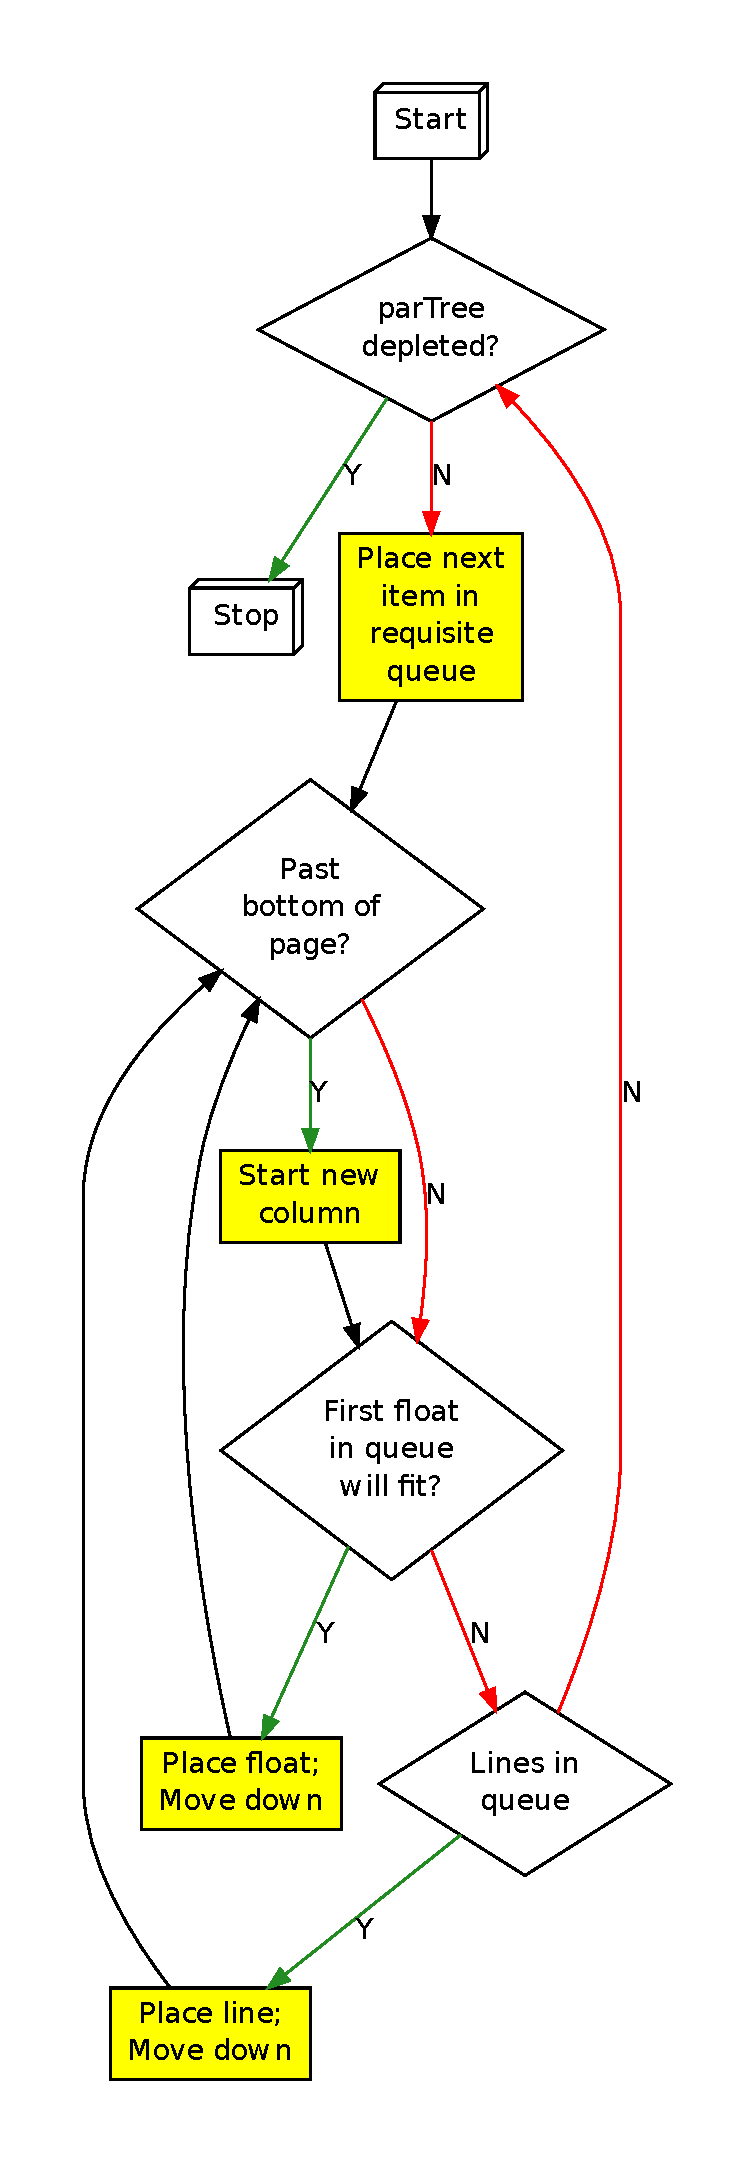
\includegraphics[height=\textheight]{gfx/floatqueueflowchart}
  \end{center}
  \caption{Flowchart describing the two-queue float algorithm}
  \label{fig:float-flowchart}
\end{figure}


Whilst this approach does produce reasonable layouts, and handles floats well without the need for backtracking, it is not particularly conducive to producing layouts with floats that span multiple columns. The queue-based layout described above is fairly dumb: although it knows about the size of each component that it lays out, it does not remember the history of the positions of any of the components it has already laid out. This makes it difficult to have items that span more than one column, because there is no mechanism to mark space on the page as being reserved. In order to do this, another approach must be taken.

\subsubsection{A Grid-Based Layout}
% - Support of floats
    % - Queue system
    % - Grid/array system (no need for queue)
    % - Multicolumn floats
        % - issues with spanning \& pagination
A simple method for allowing parts of a page to be reserved is to break it up into a grid. Many newspapers use a grid-based layout (an example is shown in figure \ref{fig:gridlayout}). Following the example set by these newspapers, the grid is defined to have a row height of the leading the document's body text, with one column in the grid per column of text.

\begin{figure}
    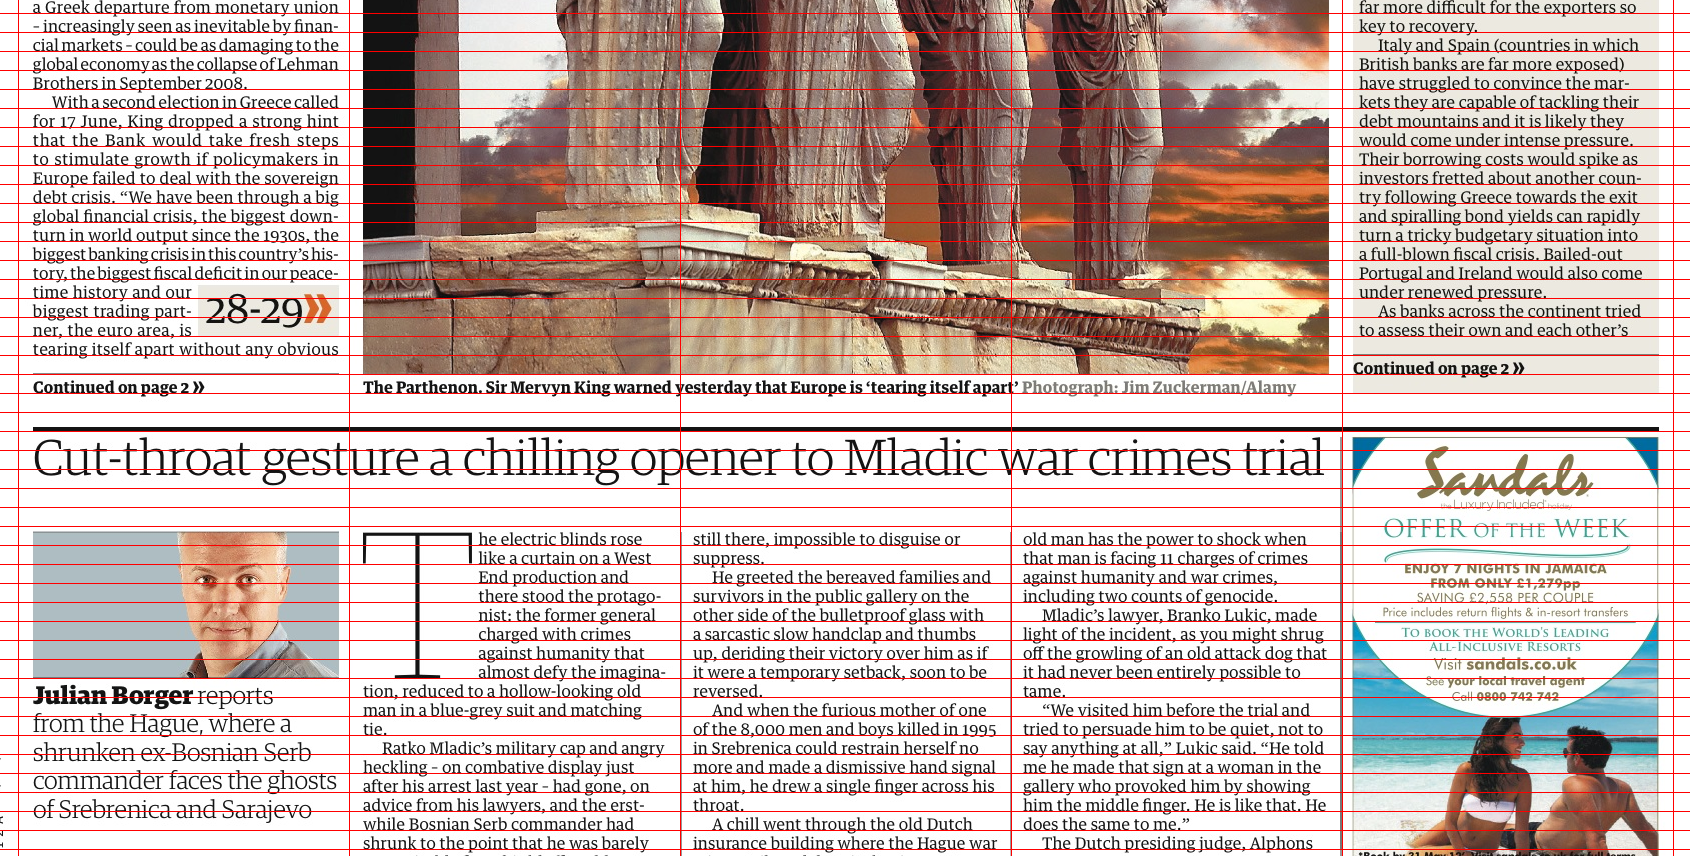
\includegraphics[width=\textwidth]{gfx/newspaper-cropped}
    \caption[An example of a grid-based layout]{An example of a grid-based layout in a UK newspaper. Note how all the baselines of the main body text are aligned to a common grid, and that all items span integer multiples of columns.}
    \label{fig:gridlayout}
\end{figure}

The viewer uses the dimensions of the float, as specified in the document structure tree (see section \ref{sec:docgen}), to determine how many columns it should span. The float is scaled to span the integer multiple of column widths that most closely matches its `natural' size, though for reasons that should hopefully be obvious, this number is limited to a minimum of 1, and a maximum of the number of columns on the page. Additionally, checks are made to ensure that the scaling will not cause height of the figure to exceed that of the page.

An advantage of this grid-based approach is that it no longer requires the use of queues, either for lines, or for floats. The viewer simply traverses the document structure tree, placing each item in the first available place in the grid. In the case of floats, or other items larger than multiples of the main leading, spaces in the grid can be marked as reserved, to prevent other items from trampling over their reserved space. If a float will not fit directly below the previous item to be placed, the grid is walked over until a sufficiently sized gap can be found. Figure~\ref{fig:screengrab} shows an example of a document laid out with our system.

\todo{Discuss pagination in detail and issues that pagination introduces for multi-column spans}

\begin{figure}
    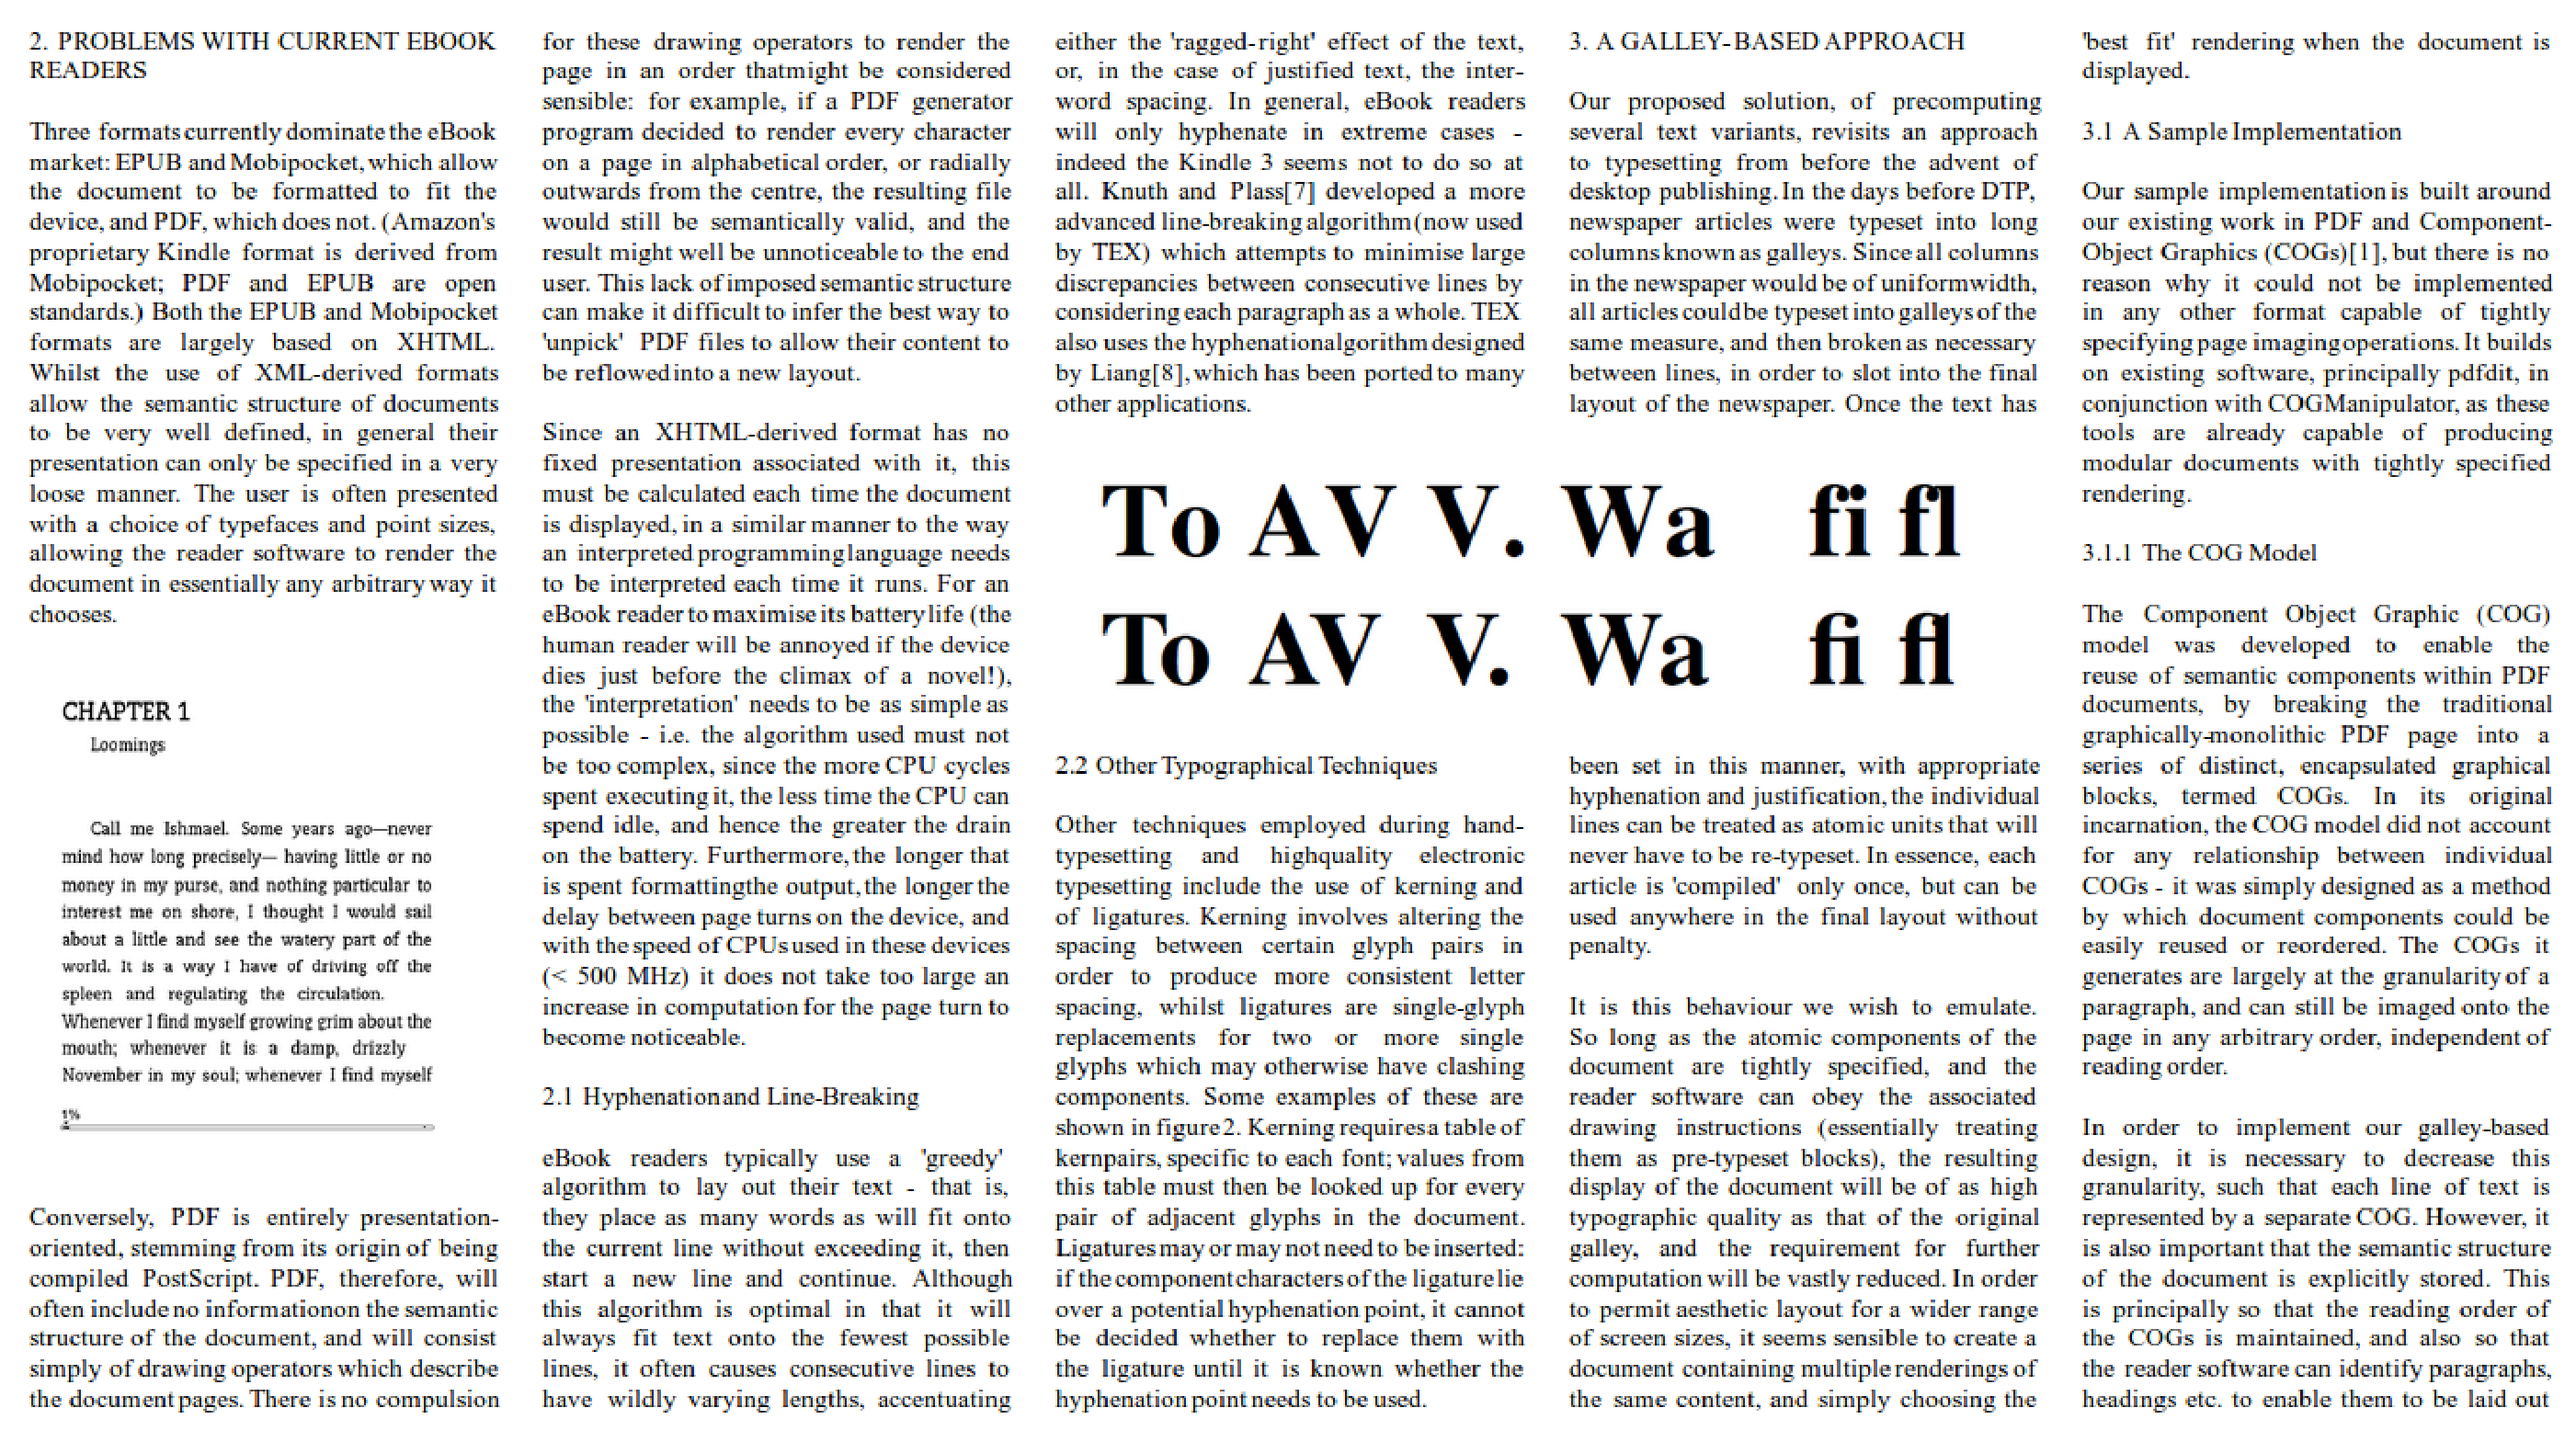
\includegraphics[width=\textwidth]{gfx/floatrendering}
    \caption[A sample rendering with multi-column floats]{An excerpt from \cite{Pinkney2011}, typeset and rendered by our new system.}
    \label{fig:screengrab}
\end{figure}

The system also supports point size changes. Although every galley is rendered in the same point size, at view time this can be scaled up or down, based on the preference of the user. The gaps between words are scaled proportionally, to allow the text to remain correctly justified.


%%%%%%%%%%%%%%%%%%%%%%%%%%%%%%%%%%%%%%%%%%%%%%%%%%


\section{Performance}
\label{sec:performance}

\subsection{Computational}
The layout system described herein works in a similar manner to a first-fit line-breaking algorithm, in that it places elements on the page in order, in the first place they will fit. Items that are the same size as a single grid cell, such as lines of text set in the main point size, can simply be placed in the first empty slot in the current column, or the first empty slot in the next column, should there be no empty spaces.  For the placement of items that are larger than a single grid cell, there is some overhead required to step through the grid until a suitable position can be found. Once a position has been found, each grid cell that it overlaps must be marked as being reserved.

Whilst this algorithm does have a greater-than-linear time complexity, the problem size is actually reduced in comparison to a first-fit text layout algorithm, since the system uses lines of text as its atomic units, rather than individual words. For this reason, it is felt that this algorithm should still be efficient enough to merit its use on portable \ebook{} readers.


    % - algorithm analysis?\\
    % - some physical timings?

\subsection{Aesthetic}
Aesthetically speaking, our system produces layouts that we feel most people would consider to be `good'. The system can guarantee use of a high-quality line breaking algorithm, since it has effectively been compiled in, and so the only remaining concern is that the columns of text and floats are laid out in a pleasing manner.

Harrington et al.~\cite{Harrington2004} identified nine aesthetic measures for automated document layout. A number of these measures (alignment, regularity, uniform separation, white-space free-flow, uniformity) are particularly well satisfied by our system, due to its use of a grid to provide regular layout.

\todo{Include picture of Greeked text that Steve printed out\ed{}mine vs web browser}
%   - Greeking\\
%       - Default browser layout vs mine\\
%       - Look at \cite{Harrington2004} for some measures and say why mine is awesome\\
%   - some discussion of choices of galley widths for best performance
    

%%%%%%%%%%%%%%%%%%%%%%%%%%%%%%%%%%%%%%%%%%%%%%%%%%



\section{Extensions}
\label{sec:future}
The system described in this chapter has only very basic support for floats. A particular limitation is that unlike paragraphs, each float has only one rendering, which must be scaled up or down as required, to fit across multiples of columns. Whilst for image-based figures or illustrations, this is probably already the desired behaviour, other types of floats, such as tables or code listings, would almost certainly benefit from the inclusion of multiple width renderings, with the choice of which rendering to display to be made at view-time. % Say that these could be differing hand-renderings, or automated from some source? Probably don't need to...

% coordinating breakpoints? might leave this until I have something sensible to say

Since the malleable document and viewer are composed entirely from HTML, CSS, and JavaScript\,---\,the core technologies behind EPUB\,---\,modifying the system to produce self-contained EPUB files seems an obvious next step.

%%%%%%%%%%%%%%%%%%%%%%%%%%%%%%%%%%%%%%%%%%%%%%%%%%
